\section{Method}


\label{sec:method}
Given an image $\x \in \mathcal{I}$, a question $\q \in \mathcal{Q}$ about the image and a set $\mathcal{A}=\{a_1,\ldots, a _K\}$ of possible answers to choose from, a \gls{vqa} model is expected to infer the answer $\hat{a} \in \mathcal{A}$ that matches the true answer $a^*$. This can be formulated as, 
\begin{equation}
    \hat{a} = \argmax_{a \in \mathcal{A}} p(a | \x,\q; \bm{\theta}),
    \label{eq:vqa}
\end{equation}
where $\bm{\theta}$ represents the parameters of the \gls{vqa} model.

% In this context, consider the relation between two QA pairs $(\q _i, a_i)$ and $(\q_j, a_j)$ for the same image $\x$ -- for example, the pairs (``Is the horse brown?", ``No") and (``What is the color of the horse?", ``White"). In this case the first pair is a necessary condition for the second one or, equivalently, the second pair is a sufficient condition for the first one.

In this context, we observe that two QA pairs $(\q _i, a_i)$ and~$(\q_j, a_j)$ for the same image~$\x$ can have different kinds of logical relations. In the simplest case, the two pairs may be unrelated, as with the pairs (``Is it nighttime?'', ``Yes'') and (``Is there a bench in the image?'', ``No''). Knowing that one of the pairs is true gives no information about the truth value of the other. 

On the other hand, two pairs may be related by a logical implication, as in the pairs (``Is the horse brown?", ``No") and (``What is the color of the horse?", ``White"). Knowing that the second pair is true implies that the first pair must be true as well. Conversely, if the first pair is false (\emph{the horse is brown}), it implies that the second pair must also be false. In this case, the first pair is a necessary condition for the second one or, equivalently, the second pair is a sufficient condition for the first one. 

Finally, it can be that two QA pairs are related by a double logical implication, as with the pairs (``Is this a vegetarian pizza?'', ``Yes'') and (``Does the pizza have meat on it?'', ``No''). The veracity of the former implies the veracity of the latter, but the veracity of the latter also implies the veracity of the former. In this case, each pair is simultaneously a necessary and sufficient condition for the other pair, and both pairs are then equivalent. 

Note that the logical implication existing between two QA pairs is an intrinsic property of the QA pairs, and does not depend on the correctness of the predictions coming from a \gls{vqa} model. If a \gls{vqa} model considers a sufficient condition true and a necessary condition false, it is incurring an \emph{inconsistency} regardless of the correctness of its predictions.
% When discussing logical implications, we will only care about the truth values of the QA pairs, but not whether the VQA model

Since logical implications are the basis of reasoning, we propose to explicitly use them when training a \gls{vqa} model to reduce its inconsistent predictions.
% If we now consider any potential pair of QAs, then four possible {logical interactions} could be observed: (1) sufficient, (2) necessary, (3) equivalent or (4) unrelated. Since these types of relationships are the basis of reasoning, we propose to explicitly use them when training a VQA model to reduce its inconsistent predictions.
Unfortunately, doing so requires overcoming two important challenges: (1)~a strategy is needed to train \gls{vqa} models with logical relations that leverage consistency in a purposeful manner. Until now, no such approach has been proposed; (2)~\gls{vqa} datasets do not typically contain logical relations between pairs of QA. Acquiring these manually would, however, be both time-consuming and difficult.

We address these challenges in this work by formalizing the idea of consistency and treating QA pairs as logical propositions from which relations can comprehensively be defined. Using this formalism, we first propose a strategy to solve (1) and train a \gls{vqa} model more effectively using logical relations and the consistency they provide~(Sec.~\ref{subsec:loss}). We then show in Sec.~\ref{subsec:relation_prediction} how we infer relations between pairs of propositions, thereby allowing standard \gls{vqa} datasets to be augmented with logical relations.

%%----------------------------$$

%\begin{figure*}[!t]
%\centering
%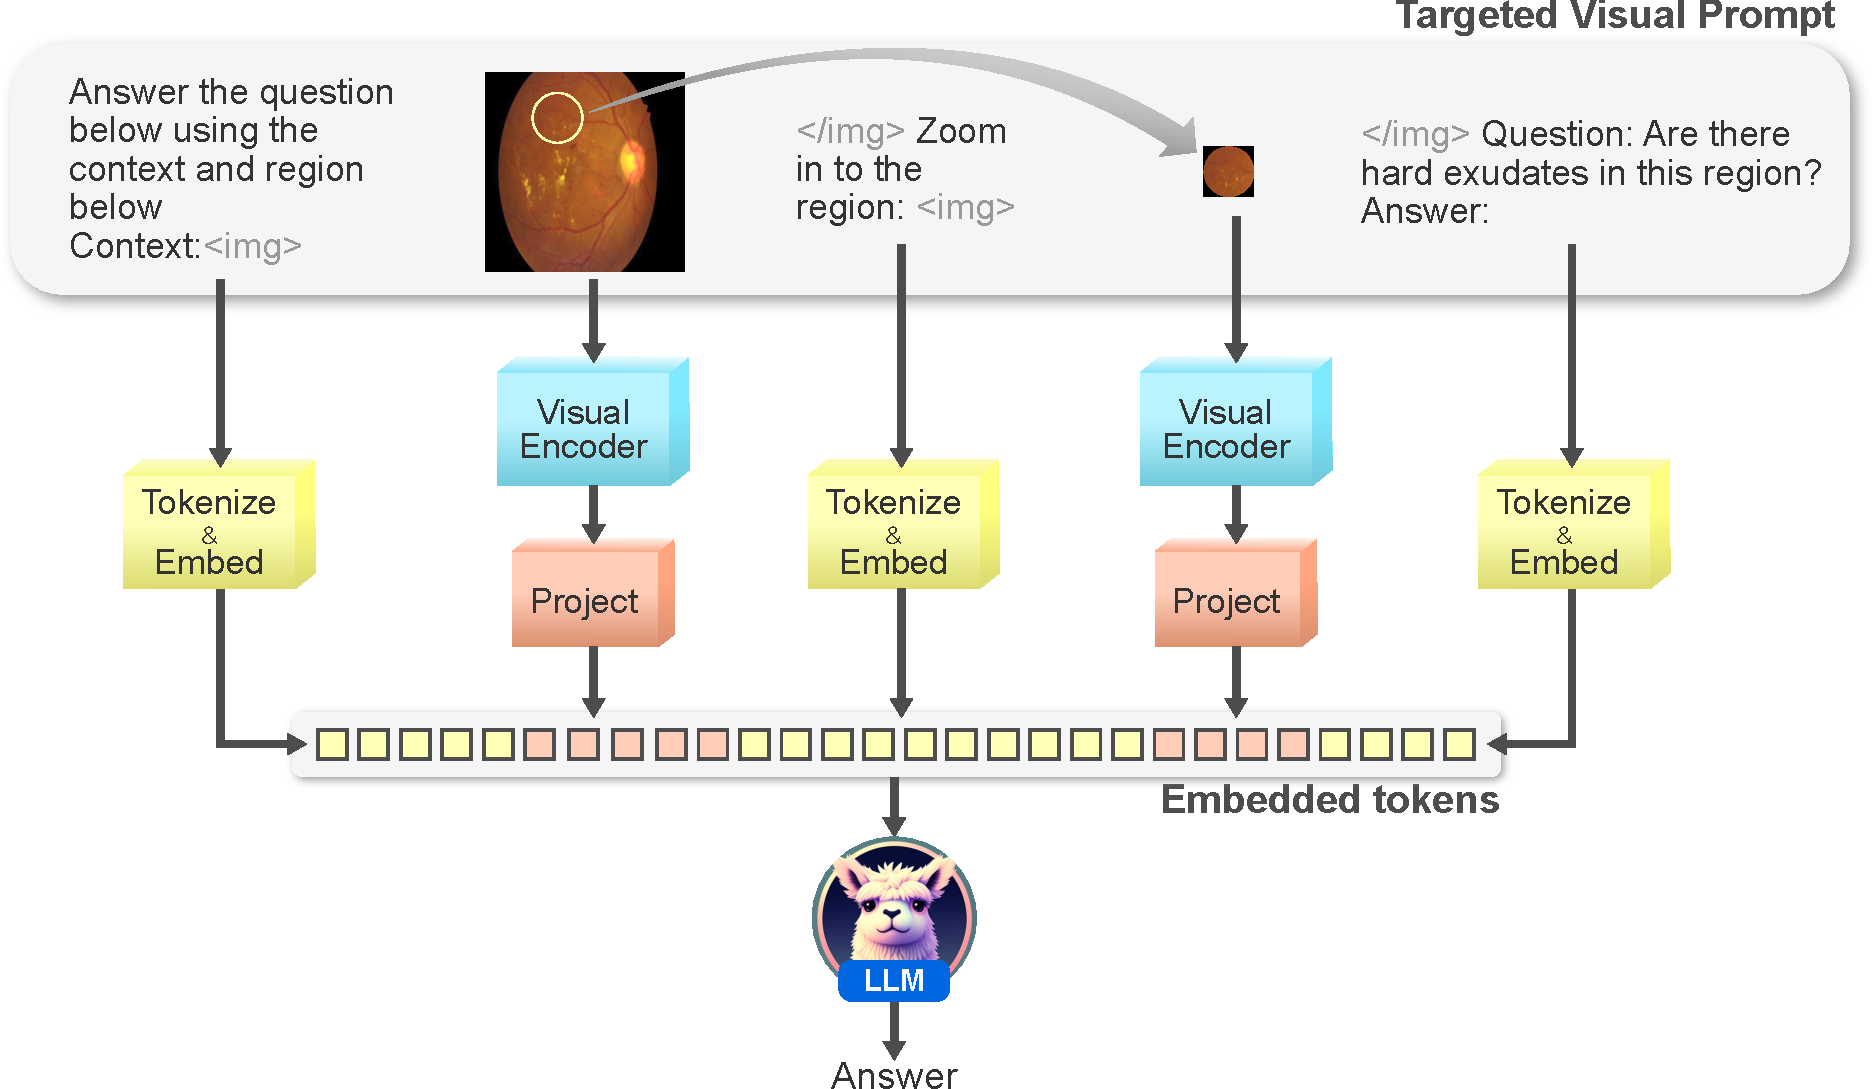
\includegraphics[width=0.85\textwidth]{images/method.pdf}
%\caption{Overview of our method. The VQA model receives a batch of images and questions that has been sampled so that related questions are consecutive. The scores provided by the model are used to compute a common VQA loss $\ell_{\textrm{VQA}}$, as well as the proposed consistency loss $\ell_{\textrm{cons}}$. For the latter, the logical implications between the pairs of question-answers are considered so as to avoid inconsistent cases.}
%\label{fig:method}
%\end{figure*}


\subsection{Consistency Formulation}
\label{subsec:consistency_framework}

We begin by observing that QA pairs~$(\q, a)$ can be considered and treated as logical propositions.
For instance, the QA (``Is it winter?", ``Yes") can be converted to ``It is winter," which is a logical proposition that can be evaluated as \emph{true} or \emph{false} (\ie,~its \emph{truth value}). Doing so allows us to use a broad definition of consistency, namely one that establishes that two propositions are inconsistent if both cannot be true at the same time~\cite{bradley1979possible}. In the context of this work, we assume the truth value of a proposition~$(\q, a)$ is determined by an agent (either a human annotator or the \gls{vqa} model) after observing the information contained in an image~$\x$. 

Let $\mathcal{D} = \mathcal{I}\times \mathcal{Q} \times \mathcal{A}$ be a \gls{vqa} dataset that contains triplets $(\x^{(n)}, \q_i^{(n)}, a_i^{(n)})$, where $\x^{(n)}$ is the $n$-th image and $(\q_i^{(n)}, a_i^{(n)})$ is the $i$-th question-answer pair about $\x^{(n)}$. In the following, we omit the index~$n$ for succinctness. For a given image $\x$, we can consider a pair of related question-answers as $(\q_i, a_i)$ and $(\q_j, a_j)$ as a pair of propositions. 
Following propositional logic notation, if both propositions are related in such a way that $(\q_i, a_i)$~is a sufficient condition for the necessary condition $(\q_j, a_j)$, we write that $(\q_i, a_i)\rightarrow (\q_j, a_j)$. For convenience, this arrow notation can be adapted to indicate different orderings between the necessary and sufficient conditions:
\begin{itemize}
    \item $(\q_i, a_i) \leftarrow (\q_j, a_j)$ if the proposition $(\q_i,a_i)$ is a necessary condition for $(\q_j,a_j)$. %: \ie, the falsity of $(\q_i,a_i)$ guarantees the falsity of $(\q_j,a_j)$.
    % \item $(\q_i, a_i) \rightarrow (\q_j, a_j)$ if the proposition $(\q_i,a_i)$ is a sufficient condition for $(\q_j,a_j)$: \ie, the truth of $(\q_i,a_i)$ guarantees the truth of $(\q_j,a_j)$. %\PMN{I'm a bit confused. Isn't $(\q_i, a_i) \rightarrow (\q_j, a_j)$ the same as $(\q_j, a_j) \leftarrow (\q_i, a_i)$? Why do we need two different arrows? Is the order of the pair of propositions important?} %\STM{It is not strictly necessary but it serves a function in the definition and using it simplifies the training so that we don't have to deal with the order of the pairs}
    \item $(\q_i, a_i) \leftrightarrow (\q_j, a_j)$ if the propositions $(\q_i,a_i)$ and $(\q_j,a_j)$ are equivalent, \ie, both are simultaneously necessary and sufficient. Note that this is just notational convenience for the double implication $(\q_i, a_i) \rightarrow (\q_j, a_j) \wedge (\q_j, a_j) \rightarrow (\q_i, a_i)$, and in the following derivations the double arrow will be always considered as two independent arrows.
    \item Finally, we will write $(\q_i, a_i) - (\q_j, a_j)$ if the propositions $(\q_i,a_i)$ and $(\q_j,a_j)$ are not related.
\end{itemize}

If a \gls{vqa} model is asked questions $\q_i$ and $\q_j$ about an image $\x$ and there exists a relation $(\q_i, a_i) \rightarrow (\q_j, a_j)$, the answers of the model will be inconsistent whenever it provides answers $\hat{a}_i = a_i$ and $\hat{a}_j \neq a_j$ (\ie, the model evaluates the first proposition as true and the second proposition as false). More generally, for a pair of necessary and sufficient conditions, the agent will be inconsistent if it evaluates the necessary condition as false and the sufficient condition as true~\cite{bradley1979possible}.
In what follows, we exploit these ideas to quantify model inconsistencies in our experiments and to develop a new loss function that encourages logically consistent \gls{vqa} models.

%%----------------------------$$
%%----------------------------$$

\subsection{Logical Implication Consistency Loss}
\label{subsec:loss}

% Additionally, given that VQAs produce a probability distribution over~$\mathcal{A}$, we can consider a probabilistic evaluation of propositions as
% \begin{equation}
%     e((\q, a), \x) = p(a\mid \x, \q, \theta),
% \end{equation}
% which, instead of the truth value of the proposition, produces the 

%  We propose a consistency loss to improve the reasoning quality of the answers provided by a VQA model. Using the consistency framework described in \ref{subsec:consistency_framework} and the annotations about relations, 


The core aim of our method is to encourage the \gls{vqa} model to avoid inconsistent answers. When training, assume that the model receives an image~$\x$ from~$\mathcal{D}$ and two associated propositions~$(\q_1, a_1)$ and~$(\q_2, a_2)$ that are related by a logical implication~$(\q_1, a_1) \rightarrow (\q_2, a_2)$. We define,
\begin{equation}
    \pi_i=\pi \left((\q_i, a_i), \x \right) = p(a_i\mid \x, \q_i; \bm{\theta}),
\end{equation}
as the probability assigned by the \gls{vqa} model that the proposition~$(\q, a)$ is true for the image~$\x$. The model has a high probability of incurring an inconsistency if it simultaneously gives a high probability~$\pi_1$ to the sufficient condition and a low probability~$\pi_2$ to the necessary condition.

We thus define our consistency loss as a function,
\begin{equation}
    \ell_\textrm{cons}(\x, (\q_1, a_1), (\q_2, a_2)) = - (1-\pi_2) \log(1-\pi_1)  - \pi_1 \log(\pi_2),
\end{equation}
that takes an image and a pair of sufficient and necessary propositions, and penalizes predictions with a high probability of inconsistency. As illustrated in \fig~\ref{fig:loss}, $\ell_\textrm{cons}$~is designed to produce maximum penalties when $\pi_1=1$ and~$\pi_2<1$ (\ie,~when the sufficient condition is absolutely certain but the necessary condition is not), and when $\pi_2=0$ and~$\pi_1>0$ (\ie,~when the necessary condition can never be true but the sufficient condition can be true). At the same time, $\ell_\textrm{cons}$ produces minimum penalties when either $\pi_1=0$ or~$\pi_2=1$, as no inconsistency is possible when the sufficient condition is false or when the necessary condition is true. Interestingly, despite its resemblance, $\ell_\textrm{cons}$ is not a cross-entropy, as it is not an expectation over a probability distribution.

% \begin{figure}
%     \centering
%     \includegraphics[width=0.9\linewidth]{images/loss_3d.png}
%     \caption{Caption}
%     \label{fig:loss_3d}
% \end{figure}

\begin{figure}
    \centering
    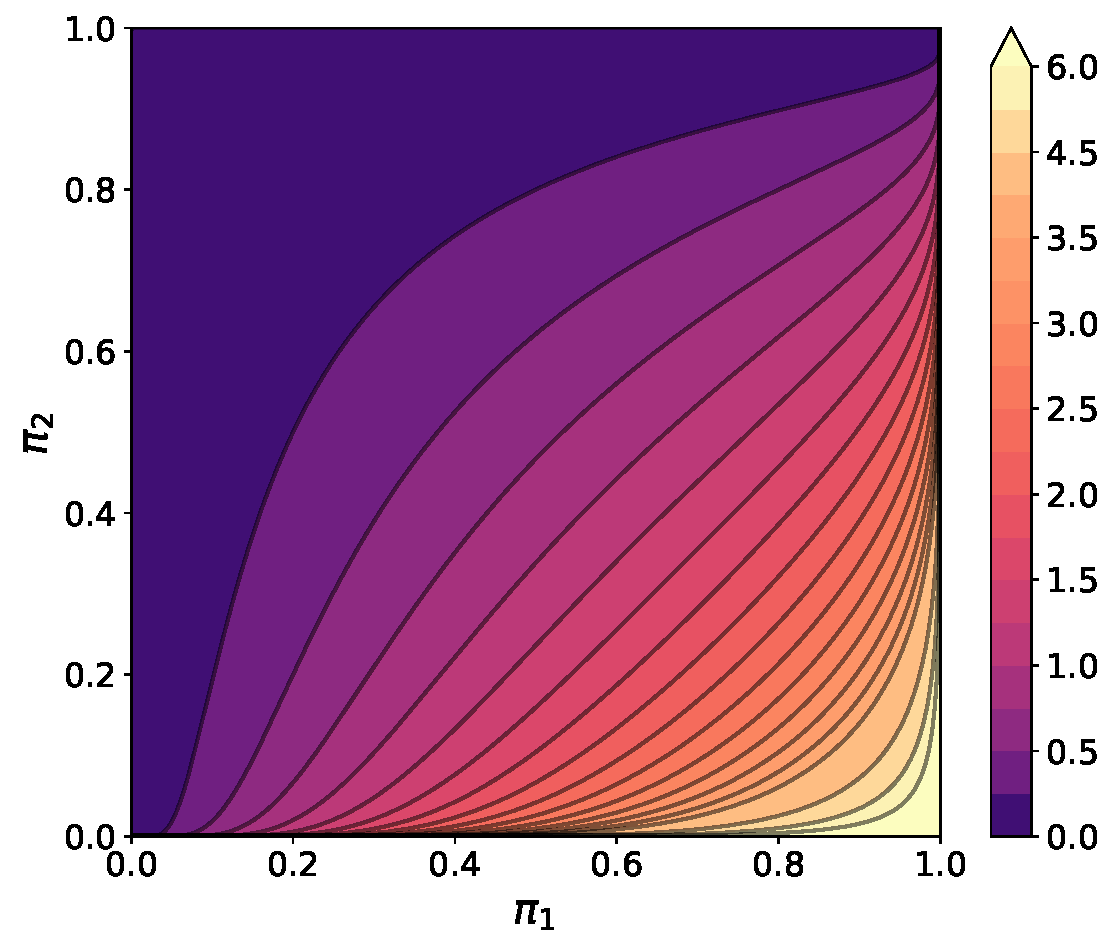
\includegraphics[width=0.5\linewidth]{Figures/Part2_Consist/02_logic/contour.pdf}
    \caption{Consistency loss~$\ell_\textrm{cons}$ as a function of the estimated probabilities for the sufficient,~$\pi_1$, and necessary,~$\pi_2$, conditions. Note that the loss diverges to~$\infty$ when $\pi_1=1, \pi_2<1$ and when~$\pi_1>0, \pi_2=0$.}
    \label{fig:loss}
\end{figure}

% Since the answers that make a pair of question-answers inconsistent depend on the relation between the pair, the value of our consistency term depends on the relation. Given a pair of questions $(\q_i, \q_j)$ about an image $\x$, with ground truth answers $(a_i, a_j)$ and model answers  $(\tilde{a}_i, \tilde{a}_j)$. Depending on the relation $r \in \{\rightarrow, \leftarrow, \leftrightarrow \}$ between $prop(\q_i, a_i)$ and $prop(\q_j, a_j)$, we define the probability terms $w$, $z$, $w^*$ and $z^*$ as shown in \ref{tab:w_z}. This terms represent the probabilities that the model gives inconsistent answers \ie the probability that a relation is violated by having a false necessary condition. For $r= \,\, \leftrightarrow$, we use $w^*$ and $z^*$ to decompose the equivalence into the combination of a necessary condition and a sufficient condition. \PMN{I do not understand these probabilities and the corresponding table. Are these the probabilities predicted by the model?} \STM{They are the probabilities of having inconsistent answers, depending on the relation. They are predicted by the model}
% \begin{table}[!t]
%   \centering
%   \begin{tabular}{@{}ccccc@{}}
%     \toprule
%     $r$ & $w$ & $z$ & $w^*$ & $z^*$  \\
%     \midrule
%     $\rightarrow$ & $p(\tilde{a}_i = a_i)$ & $p(\tilde{a}_j \neq a_j)$ & 0 & 0 \\
%     $\leftarrow$ & $p(\tilde{a}_i \neq a_i)$ & $p(\tilde{a}_j = a_j)$ & 0 & 0\\
%     $\leftrightarrow$ & $p(\tilde{a}_i = a_i)$ & $p(\tilde{a}_j \neq a_j)$ &$p(\tilde{a}_i \neq a_i)$ & $p(\tilde{a}_j = a_j)$ \\
%     \bottomrule
%   \end{tabular}
%   \caption{Probabilities of having inconsistent answers, depending on the relation between the propositions implied by the QA pairs.}
%   \label{tab:w_z}
% \end{table}

% We compute the consistency loss as shown in \ref{eq:consistency_loss}. \STM{Add justification for using this function as opposed to any other function} The intuition behind the choice of this function is the following: Since the terms $w$ and $z$ measure the probability of having inconsistent answers, we want a function that returns high values when both of these probabilities are close to one, and low values otherwise. 

% \begin{equation}
% \begin{split}
%     \ell_{\textrm{cons}}(w, z) =  -w \log (1- z) - z \log(1-w) \\ -w^* \log (1- z^*) - z^* \log(1-w^*)
%     \label{eq:consistency_loss}
% \end{split}
% \end{equation}

Our final loss is then a linear combination of the consistency loss and the cross-entropy loss $\ell_{\textrm{VQA}}$ typically used to train \gls{vqa} models. Training with this loss then optimizes, 
\begin{equation}
    \min_\theta \mathbb{E}_{\mathcal{D}}[\ell_{\textrm{VQA}}] +
    \lambda\mathbb{E}_{\substack{((\x_i, \q_i, a_i), (\x_j, \q_j, a_j))\sim\mathcal{D}^2 \\ \x_i=\x_j, (\q_i, a_i)\rightarrow (\q_j, a_j)}}[\ell_{\textrm{cons}}],
\end{equation}
where the first expectation is taken over the elements of the training set~$\mathcal{D}$ and the second expectation is taken over all pairs of necessary and sufficient propositions from~$\mathcal{D}$ defined for the same image.
In practice, we follow the sampling procedure described in~\cite{selvaraju2020squinting,tascon2022consistency}, where mini-batches contain pairs of related questions. The hyperparameter~$\lambda$ controls the relative strength between the \gls{vqa} loss and the consistency term. %\STM{Maybe in this sub-section some reviewer can wonder how we deal with equivalences (double implications)}
% \PMN{It would be a good idea either add the formula or explain what kind of loss it is (cross-entropy?)} \STM{Done}, 
% so as to optimize the performance while avoiding inconsistent answers. The total loss for training a VQA model is given by \ref{eq:total_loss}, where the hyperparameter $\lambda$ is used to adjust the relative weight of the consistency term $\ell_{\textrm{cons}}$. Our method is depicted in \ref{fig:method}.
% \begin{equation}
%     \ell_{\textrm{total}} = \ell_{\textrm{VQA}}+\lambda\ell_{\textrm{cons}}
%     \label{eq:total_loss}
% \end{equation}

%%----------------------------$$
%%----------------------------$$

\subsection{Inferring Implications}
\label{subsec:relation_prediction}
By and large, \gls{vqa} datasets do not include annotations with logical relations between question-answers pairs, which makes training a \gls{vqa} with $\ell_{\textrm{cons}}$ infeasible. To overcome this, we propose to train a language model to predict logical implications directly and use these predictions instead. We achieve this in two phases illustrated in \fig~\ref{fig:relation_prediction} and refer to our approach as the Logical-Implication model (LI-MOD).

\begin{figure}[!t]
\centering
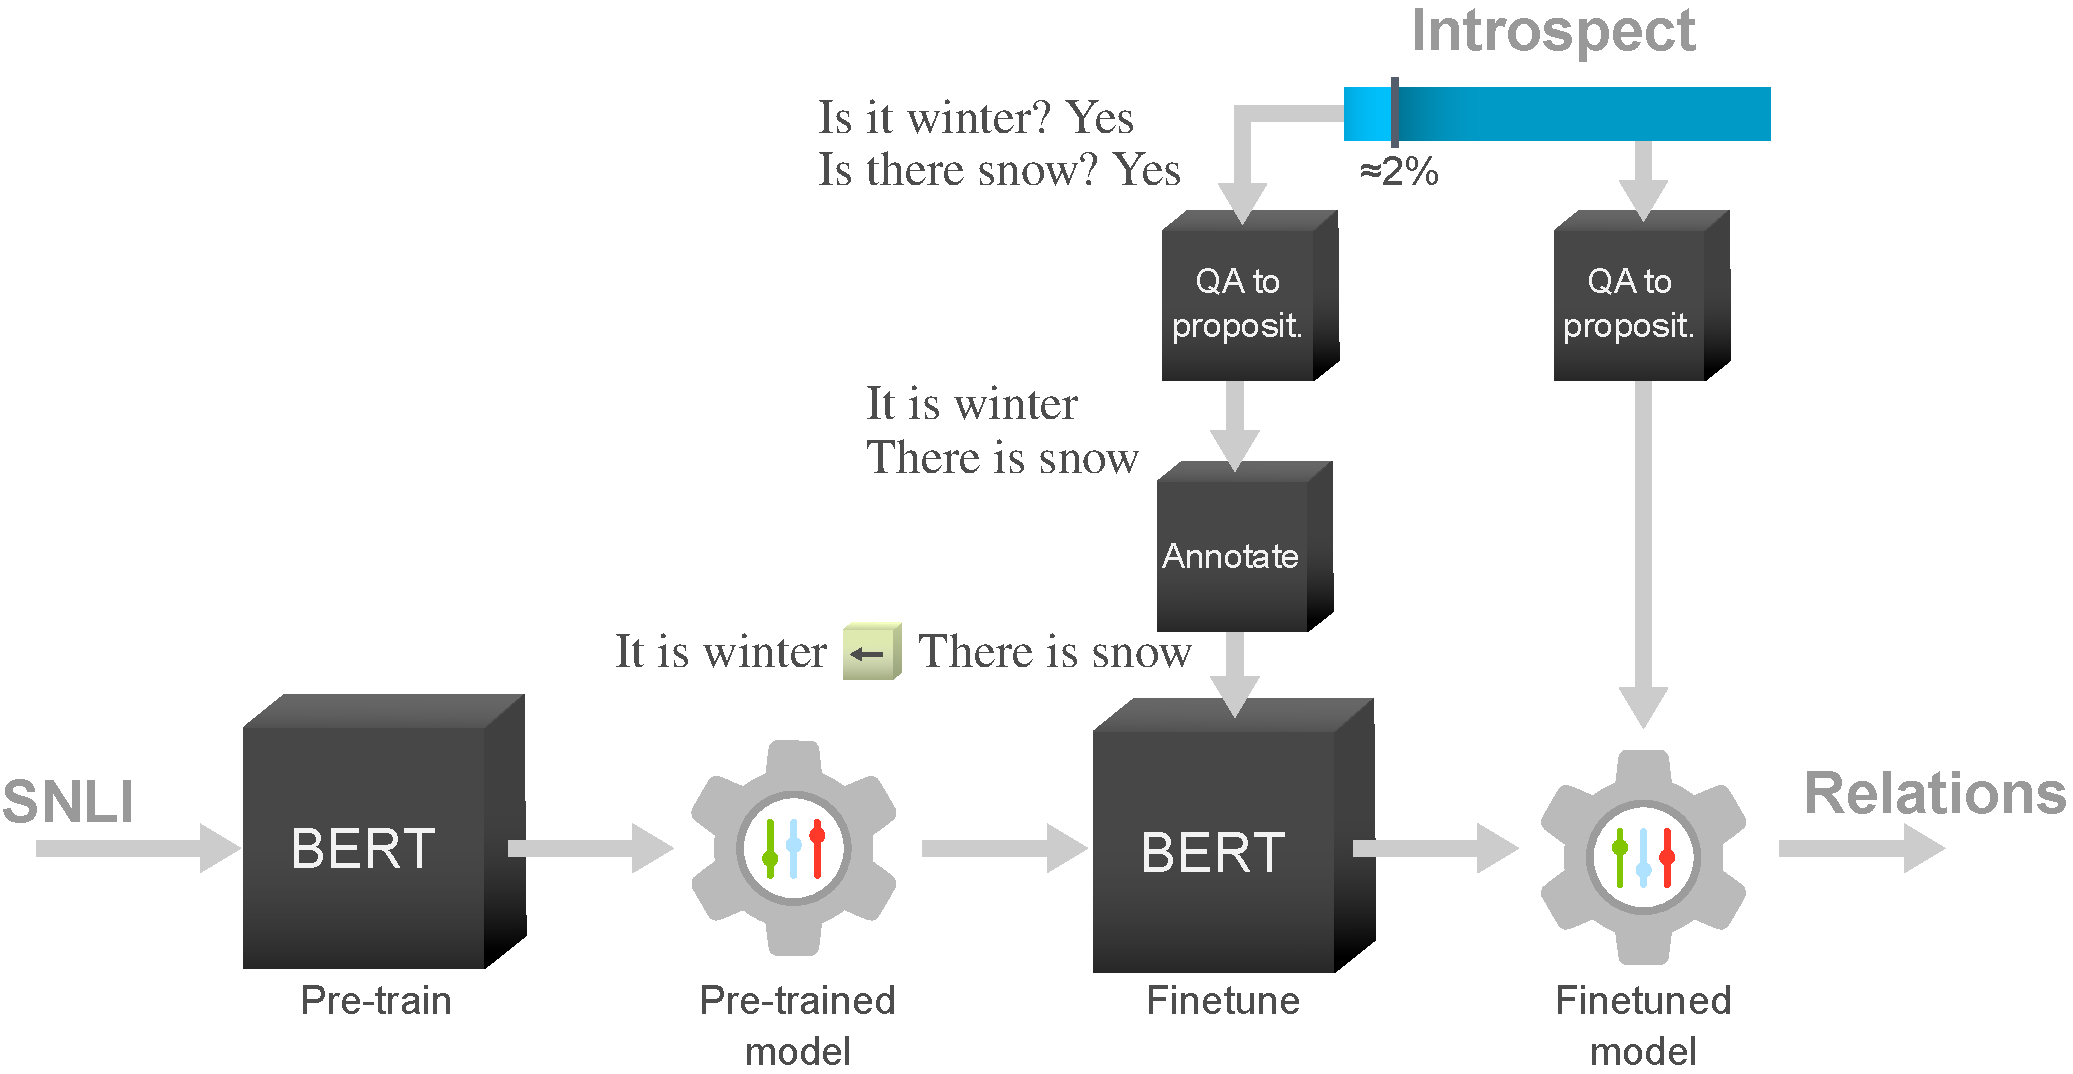
\includegraphics[width=0.7\textwidth]{Figures/Part2_Consist/02_logic/bert_relations.pdf}
    \caption{LI-MOD: Approach to predict logical relations between pairs of propositions. A BERT-based NLP model is first pre-trained on the SNLI dataset~\cite{young2014image} to solve a Natural Language Inference task and subsequently fine-tuned with annotated pairs from a subset of Introspect dataset~\cite{selvaraju2020squinting}. The resulting model is used to predict the relations of the remaining part of the dataset.}
\label{fig:relation_prediction}
\end{figure}

First, we pre-train \gls{bert}~\cite{devlin2018bert} on the task of Natural Language Inference using the SNLI dataset~\cite{young2014image}, which consists of pairs of sentences with annotations of entailment, contradiction or neutrality. In this task, given two sentences, a language model must predict one of the mentioned categories. While these categories do not exactly match the logical implication relevant to our objective, they can be derived from the entailment category. To this end, given two propositions $(\q_i,a_i)$ and $(\q_j,a_j)$, we evaluate them using the finetuned \gls{nli} model in the order $(\q_i,a_i),(\q_j,a_j)$, and then repeat the evaluation by inverting the order, to evaluate possible equivalences or inverted relations. If the relation is predicted as neutral in both passes, the pair is considered to be unrelated.

Then, we finetune the \gls{nli} model on a sub-set of annotated pairs from the \gls{vqa} dataset Introspect~\cite{selvaraju2020squinting}. In practice, we use a subset of binary QA pairs that were manually annotated with logical implications. Even though the relation need not be limited to binary questions (\ie, yes/no questions), we chose to do so because the relation annotation is simpler than for open-ended questions. Since BERT expects sentences and not QA pairs, these were first converted into propositions using Parts Of Speech (POS) tagging~\cite{petrov2011universal} and simple rules that apply to binary questions (\eg,~to convert ``Is it winter?," ``Yes" we invert the first two words of the question and remove the question mark). 
%The QA to proposition conversion is followed by the annotation process, for which we built a simple interface that shows pairs and the possible relations to the user so that the adequate relation can be chosen. 
After finetuning the model, the relations were predicted for the remaining part of the dataset. Further implementation details on this are given in~\ref{subsec:imp_details}.
